\section{Ejercicio 2}
\subsection{El Problema}

Se tienen $A$ acciones y sus valores a lo largo de $D$ días consecutivos. Se quiere saber cual es la mínima cantidad de gráficos en los que se pueden poner dichas acciones de forma tal que no se crucen las líneas ni se toquen en ningún punto y que cada acción esté en un único gráfico. Se pide un algoritmo que resuelva el problema en complejidad del orden de $O(A^2 * (A+D))$.

\subsection{Desarrollo}
Antes de comenzar, algunas definiciones:
\begin{itemize}
	\item $P(A_{i},D_{k})$ define el precio de la acción $A_{i}$ al día $D_{k}$.
	\item $A_{i} > A_{j} \Leftrightarrow (\forall d \in D) P(A_{i},d) > P(A_{j},d)$, que define un orden parcial para las acciones.
\end{itemize}
A partir del mencionado orden parcial, pudimos obtener un DAG transitivo.

Por ejemplo, considerar el siguiente caso donde se tienen cuatro acciones y sus respectivos valores a lo largo de 3 días.\\

\begin{center}
\begin{tabular}{|c|c|c|c|}
	\hline
	Acciones & \multicolumn{3}{c|}{Días}\\
	\cline{2-4}
	& 1$^{\circ}$ & 2$^{\circ}$ & 3$^{\circ}$\\
	\hline
	\hline
	\texttt{A} & \texttt{5} & \texttt{5} & \texttt{5} \\
	\hline
	\texttt{B} & \texttt{4} & \texttt{4} & \texttt{4} \\
	\hline
	\texttt{C} & \texttt{3} & \texttt{4} & \texttt{3} \\
	\hline
	\texttt{D} & \texttt{1} & \texttt{1} & \texttt{1} \\
	\hline
\end{tabular}

\end{center}
Esto daría lugar al siguiente DAG $H$ $=$ $(V,E)$, donde $V$ $=$ $A$ y $(A_{i},A_{j}) \in E \Leftrightarrow A_{j} > A_{i}$.

\begin{figure}[H]
\centering
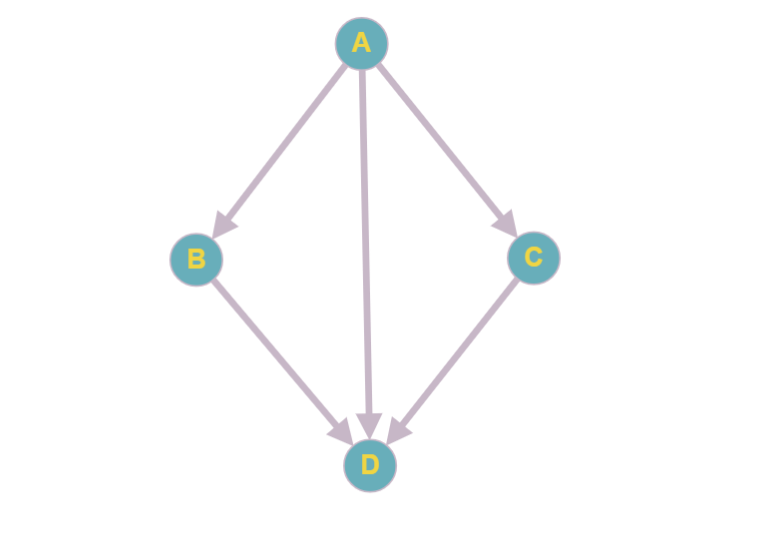
\includegraphics[width=15cm]{Imagenes/Ej2a.png}
\caption{DAG transitivo $H$}
\end{figure}

Se puede observar que un camino en este nuevo grafo consiste de acciones que pueden ir por arriba una de otra. Por ejemplo, A puede ir por arriba de B y B puede ir por arriba de D. Esto significa que pueden ir juntas en un mismo gráfico. Entonces, los caminos en el nuevo DAG ilustran grupos de acciones que pueden ir juntas.

También se puede observar que una anticadena en este grafo consiste de acciones que se tocan en algún punto. Es decir, cada vértice de una anticadena debe ir en un gráfico distinto. Se puede ver entonces que va a ser necesario usar tantos gráficos como la anticadena de tamaño máximo.

El teorema de Dilworth dice que el tamaño de la máxima anticadena es igual a la cantidad de caminos en un cubrimiento mínimo por caminos disjuntos en vértices. De esta forma se resuelve el problema. Como se dijo previamente, un camino en el DAG son acciones que pueden ir juntas. Entonces, si se obtiene un cubrimiento por caminos disjuntos en vértices que además sea mínimo, se estaría obteniendo la mínima cantidad de gráficos en los que se pueden dibujar todas esas acciones.

Para resolver este problema se utiliza matching máximo en un grafo bipartito. Para esto se construye un nuevo grafo $G$ $=$ $(IZQ,DER,E)$, donde $IZQ$ $=$ $DER$ $=$ $A$, y $(\forall A_{i}, A_{j} \in A) (A_{i}, A_{j}) \in E_{H} \Rightarrow (A_{i}, A_{j}) \in E_{G}$, con $A_{i} \in IZQ$ y $A_{j} \in DER$.\\
Así surge el siguiente grafo bipartito.

\begin{figure}[H]
\centering
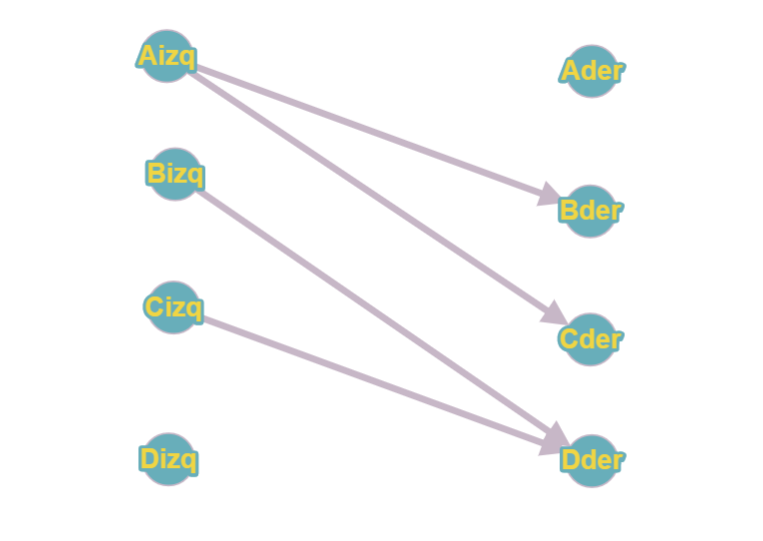
\includegraphics[width=15cm]{Imagenes/Ej2b.png}
\caption{Grafo Bipartito $G$}
\end{figure}

Si se busca un matching máximo $M$ en el siguiente grafo, se verá que es de cardinalidad 2. Uno de estos matchings posibles es $M = \{(A_{izq}, B_{der}),(C_{izq}, D_{der})\}$. Se adjunta una imagen del matching en cuestión. 

\begin{figure}[H]
\centering
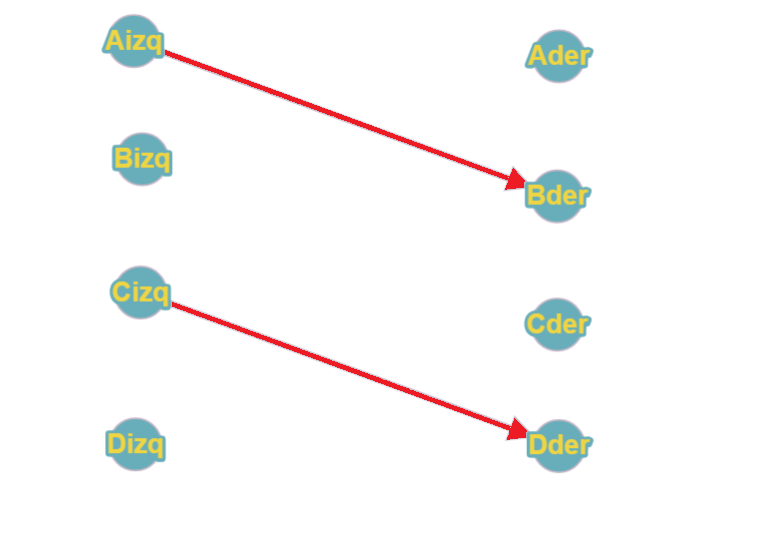
\includegraphics[width=15cm]{Imagenes/Ej2c.png}
\caption{Matching $M$ de $G$}
\end{figure}

Se puede observar que cada vértice de $IZQ$ que no tiene ningun eje en el matching, como $B_{izq}$ y $D_{izq}$, se corresponden con el último vértice de un camino en el DAG $H$. Para el caso de $B$, es el camino $A-B$ y para el caso de $D$, el camino es $C-D$. Si se hubiera elegido otro matching, como $A_{izq} - B_{der}$ y $B_{izq} - D_{der}$, los caminos representados serían $A-B-D$ y $C$.

Entonces, la cantidad de vértices de $IZQ$ del grafo $G$ que no tienen ningun eje en el matching (esto es, la cantidad de vértices de la partición menos el tamaño del matching máximo encontrado) se corresponde con la cantidad de caminos de un cubrimiento por caminos disjuntos en vértices del DAG $H$. Entonces, al maximizar el matching, se minimiza la cantidad de caminos. Por lo tanto, resolver matching máximo en el grafo $G$ resuelve el problema de encontrar mínimo cubrimiento por caminos disjuntos en vértices en el DAG $H$.

El matching bipartito, a su vez, se resuelve utilizando flujo como fue visto en clase. Se conecta una fuente a todos los vértices de la partición $IZQ$ y se conecta todos los vértices de la partición $DER$ a un sumidero, poniendole a todos los ejes capacidad 1.

\subsubsection{Complejidad}
Nuestro algoritmo consta de las siguientes partes partes:
\begin{itemize}
	\item Lectura de la entrada: Se leen $A$ acciones y por cada acción, el valor correspondiente al \emph{i-ésimo} día. Complejidad: \O{A*D}.
	\item Armado del grafo: Al momento de armar el grafo, se procedió a armar directamente el grafo bipartito $G$ previamente mencionado. Para eso, se generaron $A*2+2$ nodos. $A*2$ correspondientes a los conjuntos $IZQ$ y $DER$ de vértices, más la fuente y el sumidero. Por cada acción, se procede a ver \emph{a cuales otras acciones es mayor}, por lo que por cada accion se deben revisar todas las demás acciones y sus días. Complejidad: \O{A^2*D}.
	\item Calculo de flujo: El cálculo del flujo utilizando el algoritmo de Edmonds Karp, cuya complejidad es \O{V*E^2}. Sin embargo, al tratarse de un grafo bipartito, la complejidad es \O{V*E}\textsuperscript{\cite{cormen}}. Dado que en nuestro grafo puede haber, en peor caso, $A-1$ ejes, la complejidad es \O{A^2}.
\end{itemize}

Por propiedad de la \emph{cota asintótica superior}, la complejidad total de la solución es \O{A^2*D}